\documentclass[11pt]{article}
\usepackage[letterpaper,margin=0.9in]{geometry}
\usepackage[T1]{fontenc}
\usepackage{lmodern,amsmath,amssymb,amsthm,mathtools,microtype,tikz,enumitem,booktabs,xurl}
\usepackage[colorlinks=true,linkcolor=black,citecolor=black,urlcolor=blue!45!black]{hyperref}
\setlength{\parindent}{0pt}
\setlength{\parskip}{5pt plus 1pt minus 1pt}
\setlength{\emergencystretch}{2em}
\setlist{nosep,leftmargin=1.5em,topsep=4pt}
\newtheorem{theorem}{Theorem}[section]
\newtheorem{lemma}[theorem]{Lemma}
\newtheorem{proposition}[theorem]{Proposition}
\newtheorem{corollary}[theorem]{Corollary}
\theoremstyle{definition}
\newtheorem{definition}[theorem]{Definition}
\newcommand{\Z}{\mathbb Z}
\newcommand{\R}{\mathbb R}
\newcommand{\intr}{\operatorname{int}}
\newcommand{\dist}{\operatorname{dist}}
\newcommand{\lcm}{\operatorname{lcm}}
\hypersetup{pdfauthor={Daniel Wang and Peyton Wang}}

\title{Affine transport of endpoints in L-shaped billiards}
\author{Daniel Wang \and Peyton Wang}
\date{Working draft v0.1 --- November 8, 2026}
\begin{document}\maketitle
\begin{abstract}
An affine map of a billiard unfolding may move both endpoints: a regular straight segment between their images pulls back to the exact original pair. We apply this observation to an explicit vertical cylinder shear of an L-shaped room. A target congruence supplies straight seeds for every actual interior source, allowing seeds on smooth wall seams. For integer data the criterion reduces to one greatest-common-divisor divisibility test. We give exact two-reflection examples and distinguish this sufficient shear criterion from general illumination and from compression of an arbitrary already known path. This is a note about an affine mechanism and its limits; all-real L-room illumination is already covered by a broader theorem.
\end{abstract}

\section{The marked reflection unfolding}
Reflect an orthogonal polygon through its horizontal and vertical walls and glue matching edges by translations. The resulting compact reflection surface $M$ has translation charts away from its singularities. Mark by $\Sigma$ every lift of every genuine physical polygon corner, including convex corners that become regular surface points. An admissible segment avoids all of $\Sigma$, not merely the cone singularities.

A \emph{genuine affine map} is a global affine homeomorphism $F:M\to M$ with $F(\Sigma)=\Sigma$. In translation charts it has one invertible constant derivative. A piecewise affine deformation of a drawn polygon does not suffice. A straight regular seed may lie on a smooth polygon seam in $M$; the seam is a chart interface, not a surface singularity.

\begin{proposition}[Exact pair transport]\label{prop:transport}
Fix actual interior endpoint lifts $p,q$. If a finite straight regular segment $\eta$ in $M\setminus\Sigma$ joins $F(p)$ to $F(q)$, then $F^{-1}(\eta)$ joins the exact original $p,q$ and refolds to a finite corner-avoiding specular path. It is unnecessary to fix either endpoint under $F$.
\end{proposition}
\begin{proof}
The inverse is affine in every translation chart with one derivative. It takes the straight segment to a straight surface geodesic with the exact original endpoints, and preserves avoidance of $\Sigma$. Refolding through a smooth horizontal or vertical seam is precisely the equal-angle reflection law. The segment is compact and avoids the finite marked set, so seam crossings give a finite physical itinerary. A geodesic cannot glide along a physical wall for a nonzero interval after starting at an interior point: in a regular local chart, sharing a straight interval with that wall continues on its supporting geodesic back to the previous vertex, which would require a forbidden corner contact before entry from the interior. Smooth seam-aligned seeds are therefore allowed without creating a wall-gliding original path.
\end{proof}

The proposition is conditional. It does not assert the existence of a suitable global map or seed for every pair. It restores both original endpoints by the inverse, rather than replacing one endpoint by another point in a fiber.

\section{An L room and a global cylinder shear}
Let $A>a>0$ and $H>B>0$, and take
\[
 P=([0,A]\times[0,B])\cup([0,a]\times[B,H]).
\]
Its vertical cylinders in a signed reflection presentation are
\[
 C_{\mathrm{left}}:\ x\in(-a,a),\quad y\in\R/(2H\Z),
 \qquad
 C_{\mathrm{right}}:\ x\in(a,2A-a),\quad y\in\R/(2B\Z).
\]
Suppose a real number $k$ satisfies
\begin{equation}\label{eq:cylinders}
 ka/H\in\Z,\qquad k(A-a)/B\in\Z.
\end{equation}
On the cylinders define
\[
 V_k(x,y)=\begin{cases}
 (x,y+k(x+a)),&C_{\mathrm{left}},\\
 (x,y+k(x-a)),&C_{\mathrm{right}}.
 \end{cases}
\]
Both derivatives equal $\left(\begin{smallmatrix}1&0\\k&1\end{smallmatrix}\right)$. Boundary shifts are respectively $0,2ka$ and $0,2k(A-a)$, full cylinder circumferences by \eqref{eq:cylinders}. The maps glue pointwise along every boundary subarc with a common derivative; $V_{-k}$ is the inverse. Convex corner lifts at $x=0$ are permuted because $ka$ is an integer multiple of $H$, and those at $x=A$ because $k(A-a)$ is a multiple of $B$. The reflex and inner roof corners are fixed on cylinder boundaries. Thus $V_k$ preserves all physical corner lifts, not just cone points. The copy involution $R_y:(x,y)\mapsto(x,-y)$ also preserves them.

\begin{figure}[htbp]\centering
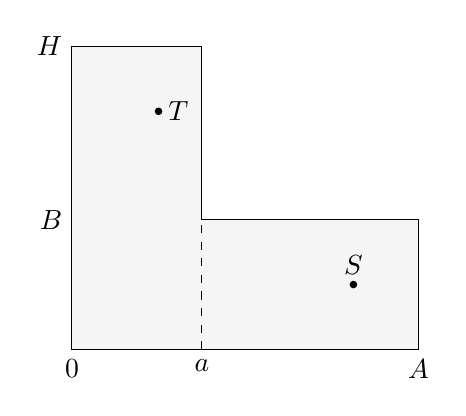
\begin{tikzpicture}[scale=.55]
\filldraw[fill=gray!8] (0,0)--(8,0)--(8,3)--(3,3)--(3,7)--(0,7)--cycle;
\draw[dashed] (3,0)--(3,3);
\fill (2,5.5) circle(2.5pt) node[right]{$T$};
\fill (6.5,1.5) circle(2.5pt) node[above]{$S$};
\node[below] at (0,0){$0$};\node[below] at (3,0){$a$};
\node[below] at (8,0){$A$};\node[left] at (0,3){$B$};\node[left] at (0,7){$H$};
\end{tikzpicture}
\caption{The L room. Sources in the left rectangle see the target directly. For sources in the right arm, the shear criterion places both endpoint images in one closed lower rectangle of the unfolding.}
\end{figure}

\section{One shear criterion for every source}
\begin{theorem}\label{thm:uniform}
Let $T=(t,v)$ with $0<t<a$ and $0<v<H$. If \eqref{eq:cylinders} holds and
\begin{equation}\label{eq:target}
 v+k(t+a)\in2H\Z,
\end{equation}
then every distinct real interior source $S$ illuminates $T$. Each right-arm source has a straight seed under either $V_k$ or $R_yV_k$.
\end{theorem}
\begin{proof}
A source with $x\le a$ sees $T$ directly in the vertical rectangle, including an actual interior point on $x=a$. Otherwise $S=(s,u)$ lies in the lower right arm, $a<s<A$, $0<u<B$. Let
\[
 r\equiv u+k(s-a)\pmod{2B},\qquad 0\le r<2B.
\]
Condition~\eqref{eq:target} sends the target to the smooth bottom point $(t,0)$. If $r\le B$, choose $F=V_k$; otherwise choose $F=R_yV_k$. Its source image in the original lower rectangle is respectively $(s,r)$ or $(s,2B-r)$. The involution fixes the target's bottom seed point.

The straight segment between the endpoint images lies in the closed lower rectangle. It avoids its bottom corners since $t>0$ and $s<A$. Any crossing of $x=a$ occurs below $B$; if the segment is horizontal on $y=0$, it stays on the smooth bottom seam away from corners. If the source image is on $y=B$, then $a<s<A$, so it lies on the smooth ledge. The segment avoids the reflex corner $(a,B)$ and all other physical corner lifts. Proposition~\ref{prop:transport} pulls it back to a legal path joining actual $S,T$. The cases $r=0$ and $r=B$ are included, without a limiting argument.
\end{proof}

The theorem isolates a uniform-source seed mechanism for targets meeting one arithmetic condition. It is not a new all-pair L-room theorem: the broader analytic illumination theorem in \cite{eightwall} already covers all real interior pairs, regardless of this condition.

\section{An exact integral criterion and its limitation}
Suppose $A,a,B,H,t,v$ are integers and restrict to integral shears $k$. Define
\[
 K=\lcm\left(\frac{H}{\gcd(a,H)},\frac{B}{\gcd(A-a,B)}\right).
\]
Condition~\eqref{eq:cylinders} holds exactly when $k=Km$, $m\in\Z$. The target condition becomes
\[
 K(t+a)m\equiv-v\pmod{2H}.
\]

\begin{corollary}\label{cor:gcd}
The integral vertical-shear criterion holds exactly when
\[
 \gcd(K(t+a),2H)\mid v.
\]
When it holds, every actual real interior source illuminates that target.
\end{corollary}
\begin{proof}
The two cylinder divisibilities yield the least common multiple $K$. A single linear congruence $cm\equiv d\pmod n$ is solvable exactly when $\gcd(c,n)$ divides $d$; a solution follows from Bezout's identity. Apply this to the displayed target congruence and then Theorem~\ref{thm:uniform}.
\end{proof}

For $(A,a,B,H)=(28,16,4,16)$ and $T=(8,8)$, one has $K=1$ and $\gcd(24,32)=8\mid8$; $k=1$ works. For $T=(8,6)$ the same full integral vertical-shear family fails because $8\nmid6$. That failure is not darkness and does not rule out other affine maps or direct analytic constructions. The exact scope is a sufficient mechanism with a complete solvability test inside its stated subfamily.

\section{Exact paths illustrating the seam cases}
In the room above with $T=(8,8)$, the following source-to-target paths all have two reflections. A listed pair of contacts is followed by the actual target.
\begin{center}\small
\begin{tabular}{@{}llll@{}}\toprule
Source & Initial direction & First contact & Second contact\\\midrule
$(26,2)$ &$(-9,7)$ &$(164/7,4)$ &$(128/7,0)$\\
$(24,2)$ &$(-8,7)$ &$(152/7,4)$ &$(120/7,0)$\\
$(22,2)$ &$(-1,1)$ &$(20,4)$ &$(16,0)$\\
$(20,2)$ &$(-6,7)$ &$(128/7,4)$ &$(104/7,0)$\\\bottomrule
\end{tabular}
\end{center}
The first source image is on the smooth ledge; the third seed is the smooth bottom-wall segment from $(22,0)$ to $(8,0)$; the fourth uses the reflected-copy branch. Each listed contact is strictly inside an actual horizontal wall. The passage line $x=16$ is crossed at respectively $16/9$, $1$, $0$ and $4/3$, all on the open passage or, for the third path, at a smooth bottom reflection before entering the left rectangle. Direct substitution verifies the equal-angle signs and final target coordinate. The zero-height case is a genuine smooth wall contact, not the reflex corner $(16,4)$.

\section{Why arbitrary path compression is a stronger question}
Pair transport proves that a suitable seed can be pulled back. It does not say that an arbitrarily selected legal path can be pushed into one polygon copy by a global affine map. The distinction is substantive: the separate noncompression result \cite{noncompression} concerns the L family
\[
 P_d=[0,2d+1]\times[0,d]\ \cup\ [0,d]\times[d,2d+1],
 \qquad d\ge3,\quad d\equiv3\pmod4,
\]
with $p=(2d-1,1)$ and $q=(1,2d-1)$. That record rules out compression of every regular connection in one specified diagonal foliation, despite an actual two-reflection path in that foliation. Its argument uses period-lattice content, cylinder-circumference ratios and a complete stabilizer calculation. Those additional classification dependencies are not proved in this note, and the result is cited only at that scoped conclusion.

Neither that fixed-foliation exclusion nor Corollary~\ref{cor:gcd}'s failed divisibility test rules out seeds obtained from another connection or a different realized affine direction. In particular no conclusion about the proposed minimum over the entire realized affine group follows here. Endpoint permutations, compatible homology matrices and local affine deformations alone are not certificates of a genuine marked global map.

\section{Source record and scope}
The complete source for the main transport and shear results is \texttt{pair-transport.md} under \path{research/illumination-generalization-2026-11-06/coordination/general-proof-priority/affine-seed-reduction/}. The four exact example paths can be checked by the repository command \texttt{python3 tools/reproduce.py affine}. This executes fixed controls; it does not establish the quantified theorem by sampling. Exact source versions are identified in the accompanying \texttt{provenance.json}.

This working note has not been externally refereed or formalized in a proof assistant. Historical novelty is unconfirmed. No all-L affine seed classification, all-ten-wall theorem or universal 22-wall minimum is asserted.

\begin{thebibliography}{9}
\bibitem{eightwall} D. Wang and P. Wang, \emph{Illumination of orthogonal rooms with at most eight walls}, working draft v0.1 (2026), included as \path{preprints/eight-wall/manuscript.pdf}.
\bibitem{noncompression} D. Wang and P. Wang, \emph{A whole connecting foliation that no full affine map can compress}, mathematical proof record (2026). The accompanying README links the full argument and its scoped reconciliation.
\end{thebibliography}

\smallskip\noindent\textbf{Acknowledgments.} The authors used AI tools, including OpenAI Codex and Anthropic Claude, to develop and revise this research, its theorem proofs, and the manuscript. The authors remain responsible for the content.
\end{document}
